\documentclass[../main.tex]{subfiles}

\begin{document}

    \section{Section I}
    \blindtext[4]\cite{texbook}

    \subsection{Sous-section I}
    \begin{wrapfigure}{r}{0.4\textwidth}
        \centering
        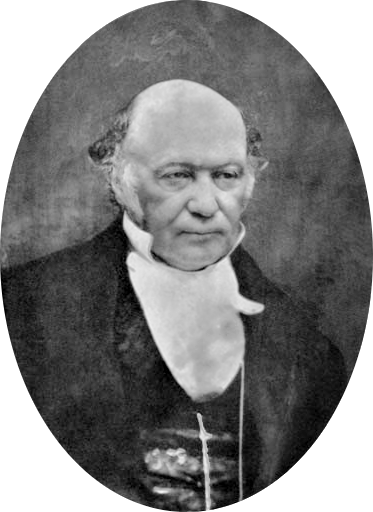
\includegraphics[scale=0.3]{figs/Hamilton_portrait.png}
        \caption{M. Hamilton.\cite{texbook}}
        \label{fig: hamilton_portrait}
    \end{wrapfigure}
    \blindtext[4]\cite{latex:companion}

    \subsubsection{Sous-sous-section I}
    \blindtext\cite{latex2e}

    \begin{table}[h!]
        \centering
        \begin{tabular}{cccc} \toprule
            $V_1$ (\V{}) & $V_2$ (\V{}) & $V_3$ (\V{}) & $V_4$ (\V{}) \\\midrule\midrule
            $290 \pm 4$ & $295 \pm 4$ & $304 \pm 4$ & $310 \pm 4$ \\
            $290 \pm 4$ & $295 \pm 4$ & $304 \pm 4$ & $310 \pm 4$ \\
            \bottomrule
        \end{tabular}
        \caption{Ajouter un texte beaucoup trop long pour être ignoré
        et beaucoup trop cours pour signigier quoique ce soit.}
        \label{table: tableau_1.1.1}
    \end{table}

    \blindtext[3]

    \begin{figure}[h!]
        \begin{center}
            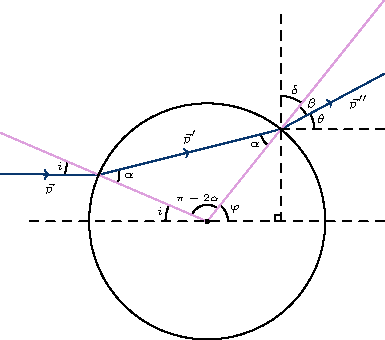
\includegraphics[width=0.6\textwidth]{figs/sphere.pdf}
        \end{center}
        \caption{Une sphère molle?}
        \label{fig: oui_une_sphere}
    \end{figure}

    \noindent
    Pour commencer cette partie du problème, on doit redéfinir les relations de conservation de la quantité de mouvement parallèle et de l'énergie. Soit
    \begin{align*}
        \Vec{p}:
        \left\{
        \begin{array}{c}
            p\sin i = p'\sin\alpha \\\\
            p'\sin\alpha = p''\sin\beta
        \end{array}
        \right.
        \betspace
        E:
        \left\{
        \begin{array}{c}
            \frac{p^2}{2m} = \frac{p'^2}{2m} + V_0 \\\\
            \frac{p'^2}{2m} + V_0 = \frac{p''^2}{2m}
        \end{array}
        \right.,
    \end{align*}

    où l'on remarque directement que $p^2 = p''^2$ et en substituant cette relation dans les équations de quantité de mouvement on trouve que
    \begin{align*}
        p\sin i = p''\sin\beta\implies\beta = i.
    \end{align*}
    Cette déduction nous permettra de trouver la relation entre les
    angles $\theta, \alpha, i$. En effet, en observant le schéma de
    la figure, on voit nécessairement que
    \begin{align*}
        \underbrace{\pi/2 = \delta + \beta + \theta}_A,\;\;\; \underbrace{\pi = i + (\pi - 2\alpha) + \varphi}_B\betspace \underbrace{\pi = \varphi + \pi/2 + \delta}_C.
    \end{align*}
    L'équation $B$ nous offre une expression pour l'angle $\varphi = 2\alpha - i$ tandis que l'équation $A$ nous offre une expression pour $\delta = \pi/2 - \beta - \theta$. En substituant ces derniers résultats dans l'équation $C$, on aura alors
    \begin{align*}
        \pi = (2\alpha - i) + \pi/2 + (\pi/2 - \beta - \theta)\implies\theta = \beta + i - 2\alpha,
    \end{align*}

    qui lorsque nous utilisons le fait que $i = \beta$, alors nous avons
    plutôt
    \begin{align*}
        \theta = 2(i - \alpha).
    \end{align*}
    À partir d'ici, nous souhaitons retrouver l'équation et pour ce
    faire, on manipulera notre dernier résultat
    \MNboxed{
        \cos\left(\frac{\theta}{2}\right) = \cos(i)\cos(\alpha) +
        \sin(i)\sin(\alpha),
    }{eq: test_eq}
    où ici nos précédente conclusions peuvent être réutilisées telles
    que l'équation ainsi que le fait
    $\sin\alpha = b/a$. \\

    \blindtext[2]

    \clearpage

\end{document}

